\documentclass[exercice]{thedocument}%
\startdatakeys
\source{}
\cycle{}
\competencesDuSocle{}
\connaissancesRequises{}
\competencesTravaillees{}
\enddatakeys
\begin{document}%
    {\bfseries Affirmation 1} : 72 est un multiple commun des nombres 12 et 18\medskip\par\noindent
    {\bfseries Affirmation 2} : pour tout nombre $n$, on a l'égalité suivante : $$(n-5)^2=n^2-5^2$$
    On considère la fonction $f$ définie par $f(x)=2x+5$.\medskip\par\noindent
    {\bfseries Affirmation 3} : l'antécédent de 6 par la fonction $f$ est égal à $\dfrac12$\medskip\par\noindent
    Voici les températures relevées en degré Celsius pendant six jours
    dans une même ville :\par
    5 $^\circ\text{C}$, 7 $^\circ\text{C}$, 11 $^\circ\text{C}$, 8 $^\circ\text{C}$, 5 $^\circ\text{C}$ et 6 $^\circ\text{C}$.\medskip\par\noindent
    {\bfseries Affirmation 4 :} la moyenne de ces températures est égale à 6,5 $^\circ\text{C}$.\medskip\par\noindent
    \begin{minipage}[t]{.5\linewidth}
        Les points B, D et A sont alignés.\par
        Les points B, E et C sont alignés.\par
        Le triangle ABC est rectangle en B.\par
        BA = 12 cm ; BC = 9 cm\par
        BD = 8 cm et BE = 6 cm.\par
        {\itshape La figure ci-contre n'est pas à l'échelle.}
    \end{minipage}\hskip20pt
    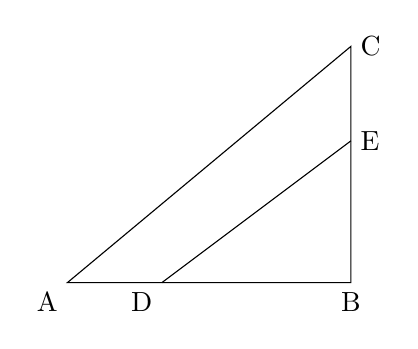
\begin{tikzpicture}[scale=0.6,baseline=(O.base)]
        \coordinate(O)at(0,2);
        \coordinate[label=below left:A](A)at(0,0);
        \coordinate[label=below left:D](D)at(2,0);
        \coordinate[label=below:B](B)at(6,0);
        \coordinate[label=right:E](E)at(6,3);
        \coordinate[label=right:C](C)at(6,5);
        \draw(A)--(B)--(C)--cycle;
        \draw(D)--(E);
    \end{tikzpicture}\medskip\par\noindent
    {\bfseries Affirmation 5} : la longueur AC est égale à 15 cm.\medskip\par\noindent
    {\bfseries Affirmation 6} : les droites (AC) et (DE) sont parallèles.
\end{document}
